% !TeX root = ../../main.tex
\question{مدل‌های گرافیکی احتمالی (\lr{PGM})}
\label{sec:question1}

% =========================================================================
% بخش اول: تحلیل سامانه پایش خرابی
% =========================================================================
\subsection{بخش اول: تحلیل سامانه پایش خرابی دستگاه‌های صنعتی}
\label{sec:q1-fault-system}

در این بخش، یک سامانه پایش خرابی دستگاه‌های صنعتی با شش متغیر تصادفی زیر مدل‌سازی می‌شود:
\begin{itemize}
  \item $F$: وقوع خرابی واقعی در دستگاه (\lr{Fault})
  \item $M$: وجود خطا در پیکربندی سامانه نگهداری (\lr{Misconfiguration})
  \item $A$: فعال‌شدن هشدار (\lr{Alarm})
  \item $Q$: میزان ازدحام صف درخواست‌های تعمیراتی (\lr{Queue Congestion})
  \item $T$: اعزام تکنسین برای بررسی هشدار (\lr{Technician Dispatch})
  \item $S$: ثبت نشانه مشخص از خرابی در گزارش بازرسی (\lr{Symptom Recorded})
\end{itemize}
متغیرهای $F$، $M$ و $Q$ متغیرهای ریشه‌ای بوده و از نظر آماری از یکدیگر مستقلند.

\subsubsection{زیربخش اول}

\textbf{۱. رسم گراف جهت‌دار بی‌دور (\lr{DAG}):} \\
بر اساس سازوکار علّی سامانه:
\begin{itemize}
  \item هشدار $A$ مستقیماً توسط خرابی واقعی $F$ و خطای پیکربندی $M$ ایجاد می‌شود: $\mathrm{Pa}(A) = \{F, M\}$.
  \item تصمیم اعزام $T$ مستقیماً بر اساس هشدار $A$ و ازدحام صف $Q$ اتخاذ می‌شود: $\mathrm{Pa}(T) = \{A, Q\}$.
  \item ثبت نشانه $S$ در گزارش بازرسی منحصراً به وقوع خرابی واقعی $F$ وابسته است: $\mathrm{Pa}(S) = \{F\}$.
  \item هیچ رابطه علّی مستقیم دیگری وجود ندارد.
\end{itemize}

مجموعه یال‌های جهت‌دار:
\[
  E = \{ F \to A, \quad M \to A, \quad F \to S, \quad A \to T, \quad Q \to T \}
\]

\begin{figure}[htbp]
  \centering
  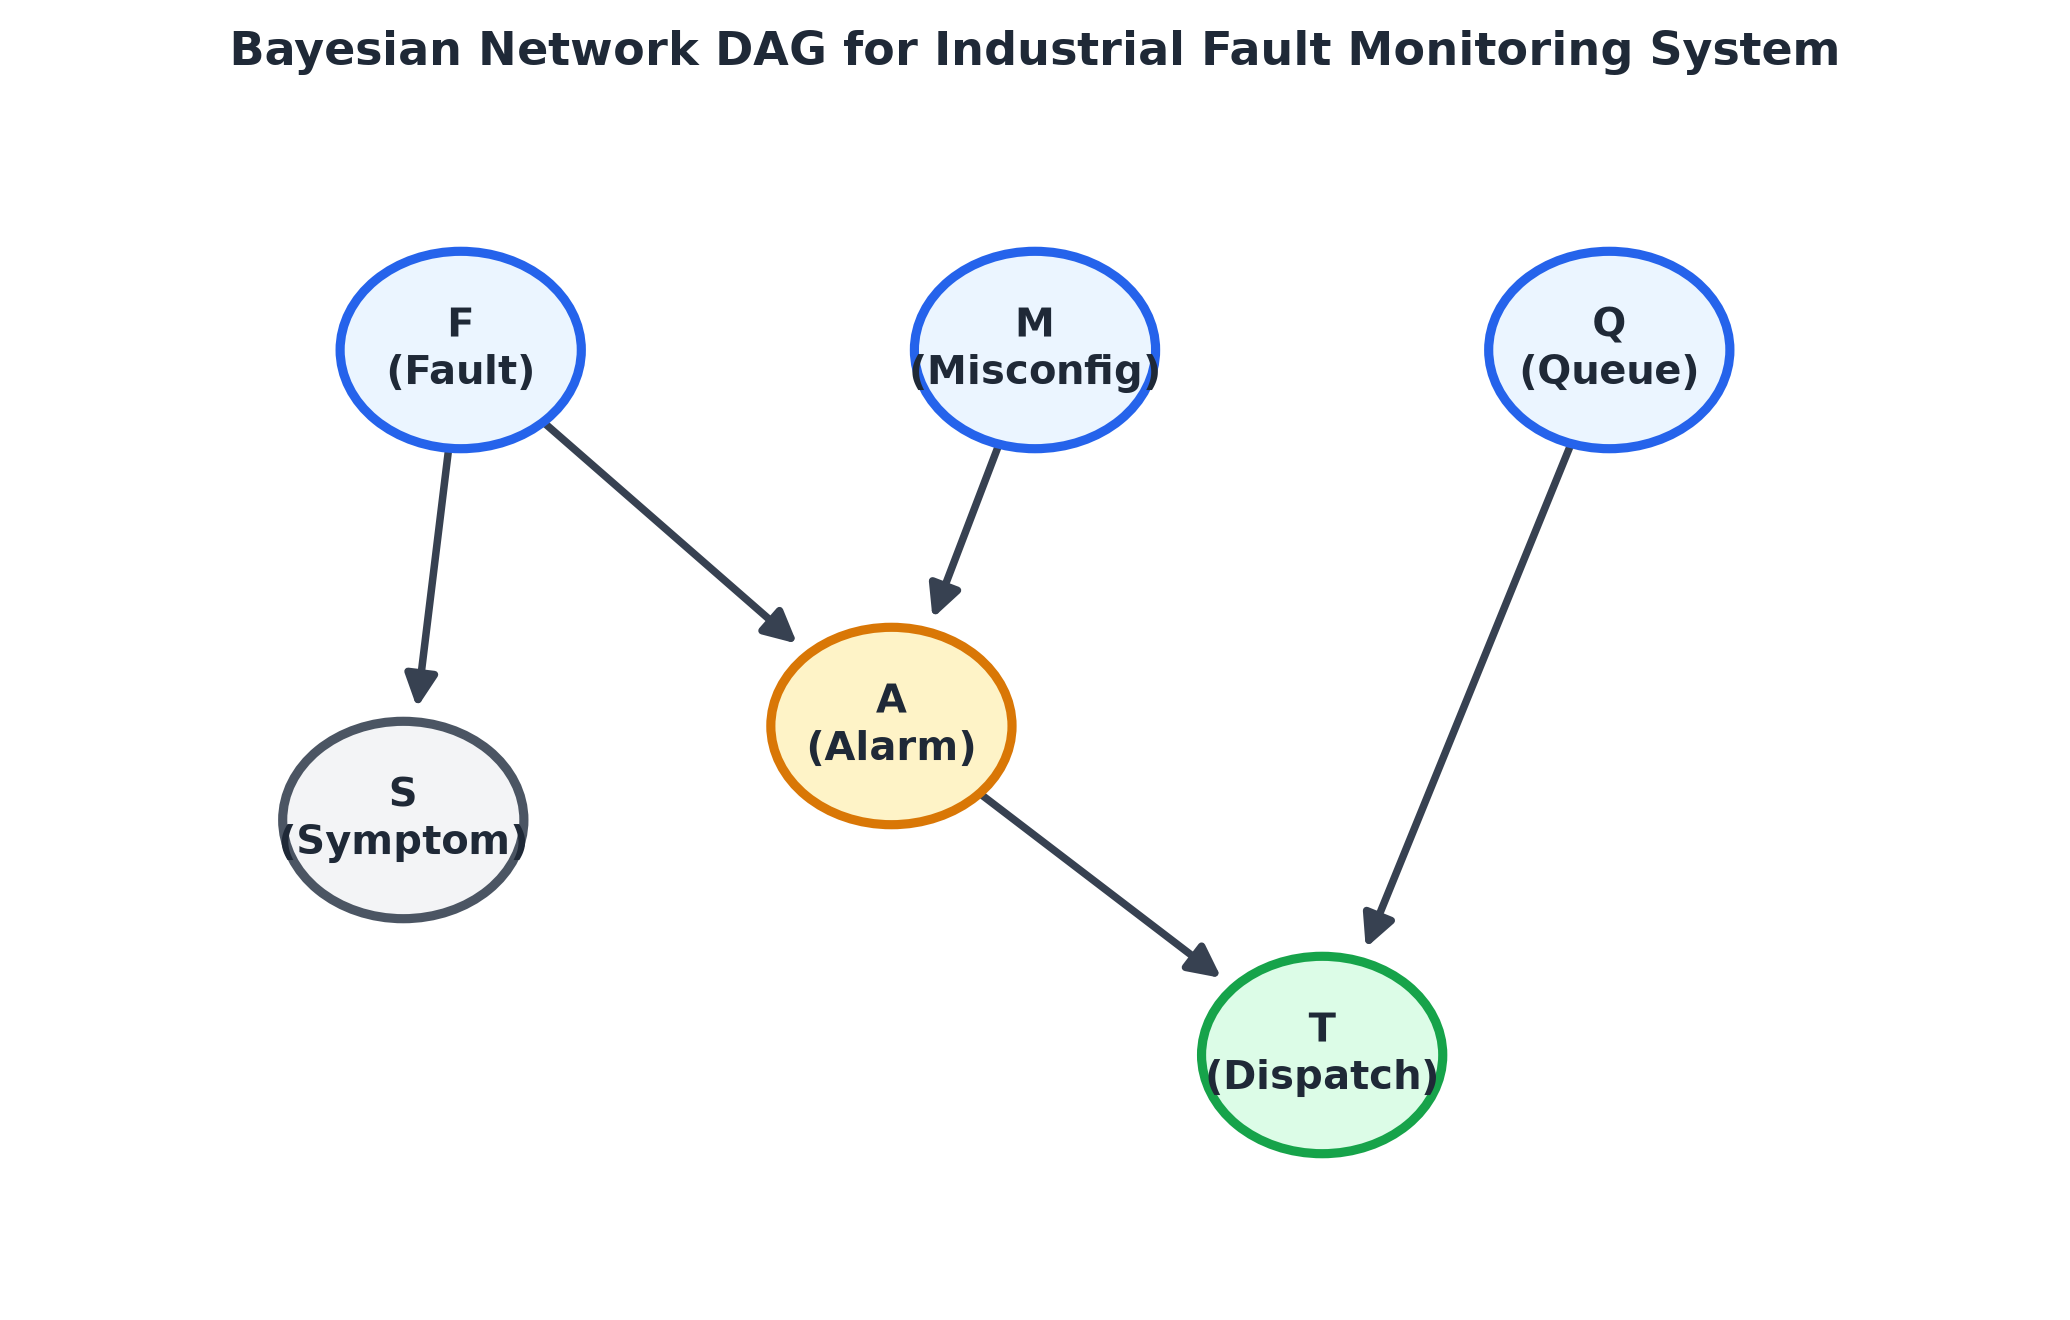
\includegraphics[width=0.72\linewidth]{problems/question1/results/q1_dag.png}
  \caption{گراف جهت‌دار بی‌دور (\lr{DAG}) سامانه پایش خرابی دستگاه و اعزام تکنسین.}
  \label{fig:q1-dag}
\end{figure}

تجزیه توزیع احتمال توأم بر اساس ساختار \lr{DAG}:
\begin{equation}
  P(F, M, A, Q, T, S) = P(F) P(M) P(Q) P(A \mid F, M) P(T \mid A, Q) P(S \mid F)
  \label{eq:q1-joint-dag}
\end{equation}

\textbf{۲. تعیین پوشش مارکوف (\lr{Markov Blanket}) متغیر $A$:} \\
طبق تعریف در شبکه‌های بیزی، پوشش مارکوف یک متغیر شامل والدین، فرزندان، و سایر والدینِ فرزندان آن متغیر است:
\[
  \mathrm{MB}(A) = \mathrm{Parents}(A) \cup \mathrm{Children}(A) \cup (\mathrm{Parents}(T) \setminus \{A\})
\]
\begin{itemize}
  \item والدین $A$: $\{F, M\}$
  \item فرزندان $A$: $\{T\}$
  \item سایر والدین فرزندان $A$: والد دیگر $T$ متغیر $Q$ است.
\end{itemize}
بنابراین:
\begin{equation}
  \mathrm{MB}(A) = \{F, M, T, Q\}
\end{equation}

\textbf{۳. بررسی مشاهده $S$ با معلوم بودن متغیرهای پوشش مارکوف:} \\
\textbf{پاسخ: خیر؛} مشاهده $S$ هیچ اطلاعات بیشتری درباره $A$ ارائه نمی‌دهد. \\
\textbf{توجیه:} طبق ویژگی اساسی پوشش مارکوف در شبکه‌های بیزی، با شرطی شدن بر کل اعضای پوشش مارکوف، آن متغیر از تمام متغیرهای دیگر شبکه مستقل شرطی می‌شود:
\[
  A \perp (V \setminus (\{A\} \cup \mathrm{MB}(A))) \mid \mathrm{MB}(A) \implies A \perp S \mid \{F, M, T, Q\}
\]
همچنین بر اساس معیار \lr{d-separation}، تنها مسیر میان $S$ و $A$ مسیر $S \leftarrow F \to A$ است. در این مسیر، گره $F$ یک انشعاب (\lr{Fork}) است که به دلیل حضور در پوشش مارکوف مشاهده شده و مسیر را مسدود می‌نماید. در نتیجه $P(A \mid F, M, T, Q, S) = P(A \mid F, M, T, Q)$.

\textbf{۴. بررسی درستی یا نادرستی استقلال‌های شرطی:}
\begin{enumerate}
  \item $F \perp A \mid M$ (\textbf{نادرست}): میان دو گره $F$ و $A$ یک یال مستقیم علّی وجود دارد ($F \to A$). هیچ مجموعه‌ای از متغیرها قادر به مسدود کردن یا \lr{d-separate} نمودن دو گره متصل با یال مستقیم نیست. بنابراین $F$ و $A$ حتی به شرط $M$ وابسته هستند.
  \item $A \perp Q \mid T$ (\textbf{نادرست}): ساختار $A \to T \leftarrow Q$ یک تصادم‌دهنده (\lr{Collider / v-structure}) در گره $T$ است. متغیرهای $A$ و $Q$ به صورت حاشیه‌ای مستقلند، اما با شرطی شدن بر گره تصادم‌دهنده $T$، مسیر میان آن‌ها فعال (\lr{Unblocked}) شده و به یکدیگر وابسته می‌شوند (پدیده \lr{Explaining Away}).
  \item $S \perp M \mid F$ (\textbf{درست}): مسیرهای میان $S$ و $M$ عبارتند از $S \leftarrow F \to A \leftarrow M$ که در گره $F$ (انشعاب مشاهده‌شده) مسدود است؛ همچنین در گره $A$ (تصادم‌دهنده مشاهده‌نشده) نیز مسدود است. چون تمامی مسیرها مسدود هستند، $S$ و $M$ به شرط $F$ مستقل شرطی‌اند.
\end{enumerate}

\subsubsection{زیربخش دوم}

قانون قطعی هشدار: $A = F \lor M$ با $P(F=1) = 0.2$ و $P(M=1) = 0.2$ مستقل از یکدیگر.

\textbf{۱. پیش‌بینی کیفی و پدیده احتمالاتی مربوط:} \\
متغیرهای $F$ و $M$ علل بالقوه و مستقل وقوع معلول $A$ هستند ($F \to A \leftarrow M$). پیش از مشاهده هشدار، این دو کاملاً مستقلند ($F \perp M$). اما پس از مشاهده فعال شدن هشدار ($A=1$)، می‌دانیم حداقل یکی از آن‌ها رخ داده است. حال اگر بدانیم خرابی واقعی رخ داده است ($F=1$)، وقوع هشدار کاملاً توجیه شده و ضرورت حضور خطای پیکربندی برای توضیح هشدار کاهش می‌یابد. این پدیده به «توجیه شدن علّت» (\lr{Explaining Away}) یا تناقض برکسون (\lr{Berkson's Paradox}) موسوم است؛ بنابراین متغیرها وابسته شده و همبستگی میان آن‌ها \textbf{منفی} است.

\textbf{۲. محاسبات عددی احتمالات:} \\
حالات مختلف توزیع توأم $F$ و $M$:
\begin{itemize}
  \item $P(F=0, M=0) = 0.8 \times 0.8 = 0.64 \quad (A=0)$
  \item $P(F=0, M=1) = 0.8 \times 0.2 = 0.16 \quad (A=1)$
  \item $P(F=1, M=0) = 0.2 \times 0.8 = 0.16 \quad (A=1)$
  \item $P(F=1, M=1) = 0.2 \times 0.2 = 0.04 \quad (A=1)$
\end{itemize}
احتمال کل وقوع هشدار:
\[
  P(A=1) = 1 - P(F=0, M=0) = 1 - 0.64 = 0.36
\]
\begin{itemize}
  \item \textbf{محاسبه $P(F=1 \mid A=1)$:}
  \[
    P(F=1 \mid A=1) = \frac{P(F=1, A=1)}{P(A=1)} = \frac{P(F=1)}{P(A=1)} = \frac{0.20}{0.36} = \frac{5}{9} \approx 0.5556
  \]
  \item \textbf{محاسبه $P(F=1, M=1 \mid A=1)$:}
  \[
    P(F=1, M=1 \mid A=1) = \frac{P(F=1, M=1, A=1)}{P(A=1)} = \frac{0.04}{0.36} = \frac{1}{9} \approx 0.1111
  \]
\end{itemize}

\textbf{۳. اثر آگاهی از خرابی واقعی بر احتمال خطای پیکربندی:} \\
- احتمال خطای پیکربندی صرفاً با مشاهده هشدار ($A=1$):
\[
  P(M=1 \mid A=1) = \frac{P(M=1)}{P(A=1)} = \frac{0.20}{0.36} = \frac{5}{9} \approx 0.5556
\]
- احتمال خطای پیکربندی با مشاهده هشدار و آگاهی از وقوع خرابی واقعی ($A=1, F=1$):
\[
  P(M=1 \mid A=1, F=1) = \frac{P(F=1, M=1 \mid A=1)}{P(F=1 \mid A=1)} = \frac{1/9}{5/9} = \frac{1}{5} = 0.20
\]
\textbf{مقایسه:} مشاهده می‌شود که با آگاهی از وقوع خرابی واقعی، احتمال خطای پیکربندی از $0.5556$ مجدداً به احتمال پایه $0.20$ کاهش می‌یابد که تأییدکننده همبستگی منفی و اثر \lr{Explaining Away} است.

\textbf{۴. استقلال وابسته به زمینه (\lr{Context-Specific Independence - CSI}):} \\
- \textbf{شرط استقلال:} در قانون قطعی $A = F \lor M$، در زمینه $F=1$ داریم:
\[
  (A \perp M \mid F=1)
\]
و به صورت متقارن در زمینه $M=1$ نیز $(A \perp F \mid M=1)$ برقرار است. \\
- \textbf{دلیل:} عملگر منطقی \lr{OR} دارای خاصیت جذب است ($1 \lor M = 1$). بنابراین در زمینه $F=1$، تغییر وضعیت متغیر $M$ هیچ تأثیری بر وضعیت هشدار نمی‌گذارد. \\
- \textbf{علت عدم کفایت حذف یال در DAG کلاسیک:} حذف یال $M \to A$ در یک \lr{DAG} یک استقلال عمومی سراسری ($A \perp M \mid F$) برای تمام زمینه‌ها ایجاد می‌کند؛ در حالی که وقتی $F=0$ است، مقدار هشدار مستقیماً تابع $M$ است ($A = 0 \lor M = M$). بنابراین حذف یال ادعاهای اساسی مدل را تغییر می‌دهد.

% =========================================================================
% بخش دوم: میدان‌های تصادفی مارکوفی (MRF)
% =========================================================================
\subsection{بخش دوم: میدان‌های تصادفی مارکوفی زوجی و شبکه‌های بیزی}
\label{sec:q1-mrf}

چهار زمین کشاورزی $W, X, Y, Z$ در یک دور چهار‌رأسی $W - X - Y - Z - W$ بر روی یک میدان مارکوفی زوجی با گراف بدون جهت $H$ قرار دارند.

\begin{figure}[htbp]
  \centering
  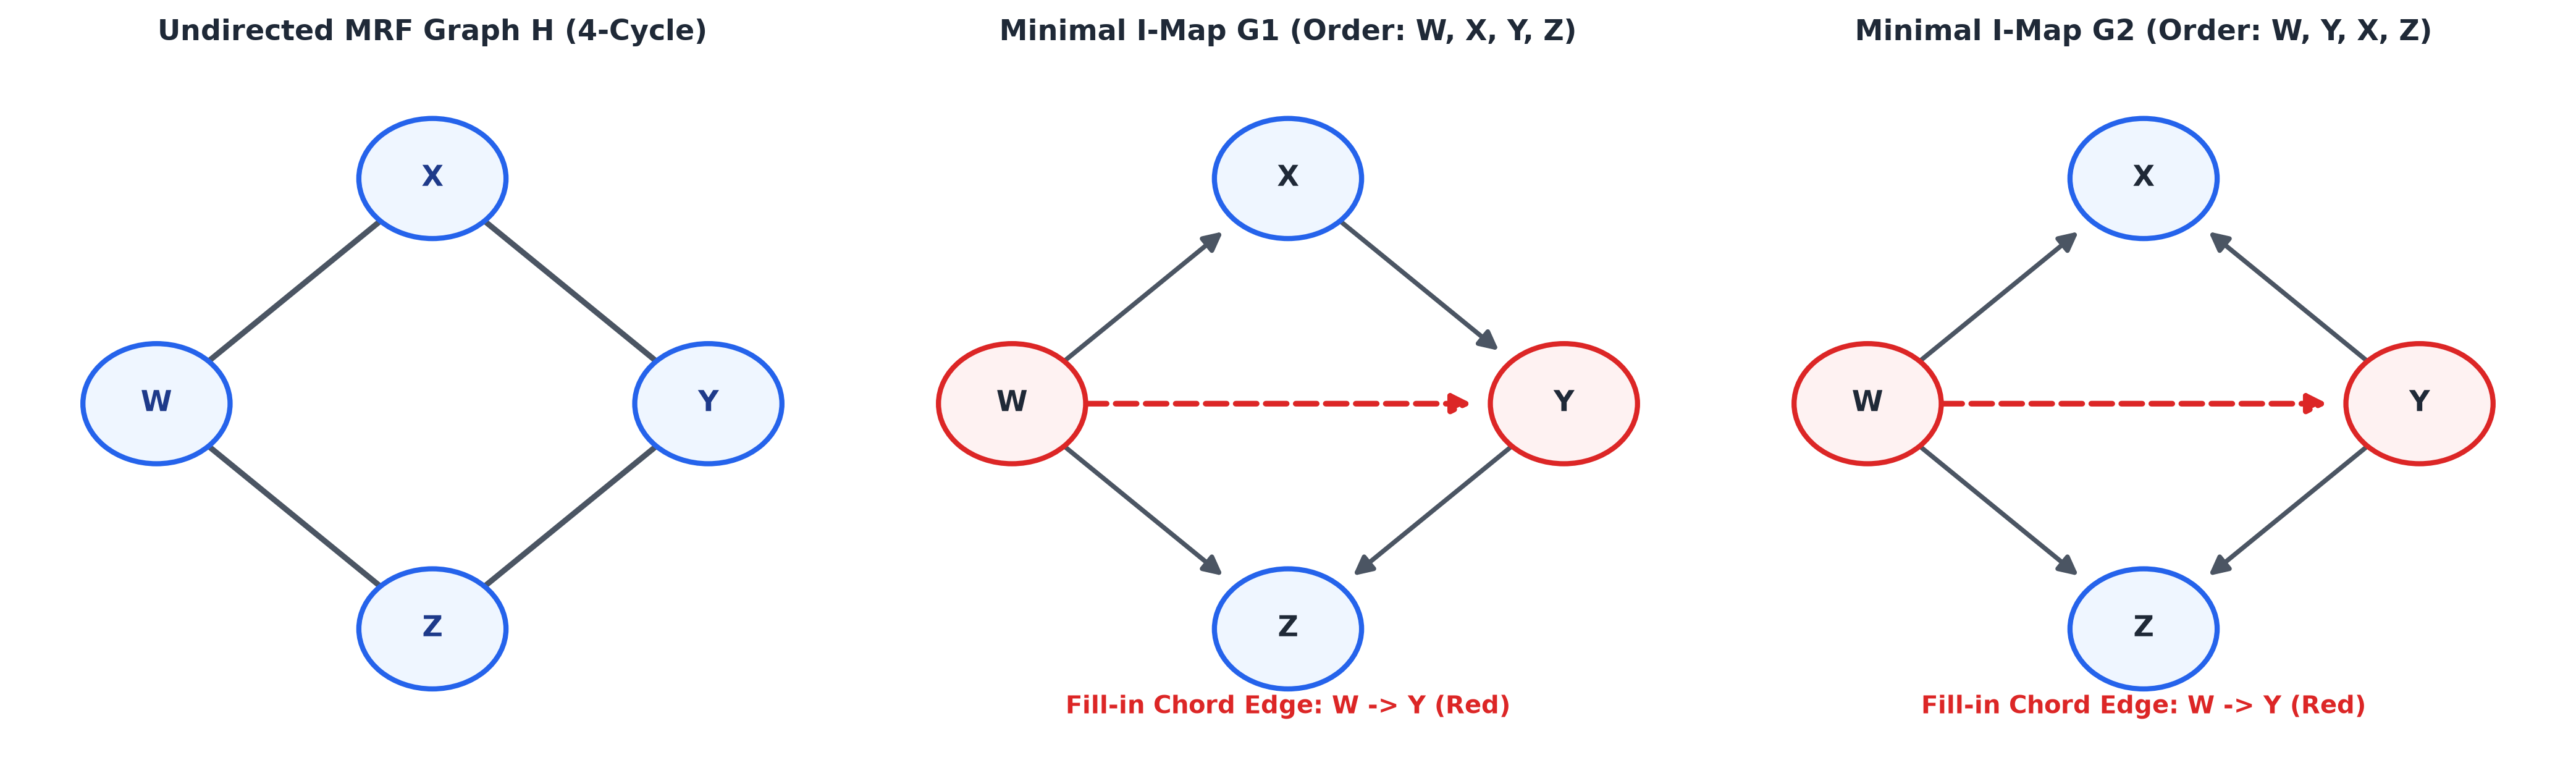
\includegraphics[width=0.95\linewidth]{problems/question1/results/q1_mrf_and_imaps.png}
  \caption{گراف بدون جهت $H$ (میدان مارکوفی زوجی ۴تایی) و نگاشت‌های استقلالی کمینه $G_1$ و $G_2$ با یال وتری تکمیلی $W \to Y$.}
  \label{fig:q1-mrf-imaps}
\end{figure}

\subsubsection{زیربخش اول}

\textbf{۱. استقلال‌های شرطی قابل استنتاج از $H$ ($I(H)$):} \\
در گراف بدون جهت $H$ (دور فاقد وتر $C_4$):
\[
  I(H) = \{ (W \perp Y \mid X, Z), \quad (X \perp Z \mid W, Y) \}
\]

\textbf{۲. ساخت نگاشت استقلالی کمینه (\lr{Minimal I-map}) از نوع DAG:}
\begin{itemize}
  \item \textbf{ترتیب اول: $W, X, Y, Z$:}
  \begin{enumerate}
    \item $W$: متغیر اول است: $\mathrm{Parents}(W) = \emptyset$.
    \item $X$: متغیر قبلی $W$ است: $\mathrm{Parents}(X) = \{W\}$.
    \item $Y$: متغیرهای قبلی $\{W, X\}$ هستند. چون $Z$ شرطی نشده، مسیر $Y-Z-W$ باز است و $Y \not\perp W \mid X$: $\mathrm{Parents}(Y) = \{W, X\}$.
    \item $Z$: متغیرهای قبلی $\{W, X, Y\}$ هستند. با داشتن $\{W, Y\}$، طبق $I(H)$ داریم $Z \perp X \mid W, Y$: $\mathrm{Parents}(Z) = \{W, Y\}$.
  \end{enumerate}
  یال‌های حاصل در $G_1$: $\{ W \to X, \quad W \to Y, \quad X \to Y, \quad W \to Z, \quad Y \to Z \}$. \\
  تجزیه توأم: $P(W, X, Y, Z) = P(W) P(X \mid W) P(Y \mid W, X) P(Z \mid W, Y)$.

  \item \textbf{ترتیب دوم: $W, Y, X, Z$:}
  \begin{enumerate}
    \item $W$: $\mathrm{Parents}(W) = \emptyset$.
    \item $Y$: متغیر قبلی $W$ است و وابسته هستند: $\mathrm{Parents}(Y) = \{W\}$.
    \item $X$: متغیرهای قبلی $\{W, Y\}$ هستند: $\mathrm{Parents}(X) = \{W, Y\}$.
    \item $Z$: متغیرهای قبلی $\{W, Y, X\}$ هستند و $Z \perp X \mid W, Y$: $\mathrm{Parents}(Z) = \{W, Y\}$.
  \end{enumerate}
  یال‌های حاصل در $G_2$: $\{ W \to Y, \quad W \to X, \quad Y \to X, \quad W \to Z, \quad Y \to Z \}$. \\
  تجزیه توأم: $P(W, X, Y, Z) = P(W) P(Y \mid W) P(X \mid W, Y) P(Z \mid W, Y)$.
\end{itemize}

\textbf{۳. بررسی هم‌ارزی استقلالی (\lr{I-Equivalence}):} \\
طبق قضیه ورما و پرل، دو \lr{DAG} هم‌ارز استقلالی هستند اگر و تنها اگر اسکلت یکسان و تصادم‌دهنده‌های غیراخلاقی (ناوتر) یکسان داشته باشند:
\begin{itemize}
  \item \textbf{اسکلت:} هر دو گراف $G_1$ و $G_2$ دارای ۵ یال بدون جهت یکسان هستند: $(W, X), (W, Y), (X, Y), (W, Z), (Y, Z)$.
  \item \textbf{تصادم‌دهنده‌ها:} در هر دو گراف، والدین گره‌های دارای دو والد به وسیله یال $W \to Y$ به یکدیگر متصل هستند؛ بنابراین هیچ تصادم‌دهنده ناوتر در هیچ‌یک وجود ندارد.
\end{itemize}
چون هر دو شرط برقرار است، دو \lr{DAG} از نظر استقلال‌های شرطی \textbf{کاملاً هم‌ارزند}: $I(G_1) = I(G_2)$.

\subsubsection{زیربخش دوم}

\textbf{اثبات عدم وجود نگاشت کامل (\lr{Perfect Map}) در DAG:} \\
یک میدان مارکوفی $H$ دارای نگاشت کامل \lr{DAG} است اگر و تنها اگر گراف $H$ وتری (\lr{Chordal / Triangulated}) باشد. \\
\textbf{اثبات تحلیلی:} در دور $C_4$، برقراری همزمان استقلال‌های $(W \perp Y \mid X, Z)$ و $(X \perp Z \mid W, Y)$ مستلزم آن است که هیچ‌یک از گره‌های $X, Z, W, Y$ تصادم‌دهنده نباشند. در یک دور ۴رأسی، فقدان تصادم‌دهنده ناگزیر یک دور جهت‌دار ($W \to X \to Y \to Z \to W$) تولید می‌کند که ناقض تعریف \lr{DAG} است. بنابراین هیچ \lr{DAG}ای نمی‌تواند نگاشت کامل برای این گراف بدون جهت باشد. $\blacksquare$

\subsubsection{زیربخش سوم}

\textbf{۱. استقلال‌های حفظ‌شده و از دست‌رفته در DAGهای ساخته‌شده:}
\begin{itemize}
  \item \textbf{استقلال حفظ‌شده:} $X \perp Z \mid W, Y$ (مسیرهای میان $X$ و $Z$ به دلیل شرطی شدن بر والدین $Z$ مسدود می‌مانند).
  \item \textbf{استقلال از دست‌رفته:} $W \perp Y \mid X, Z$ (به دلیل اضافه شدن یال مستقیم $W \to Y$ میان این دو گره).
\end{itemize}

\textbf{۲. انتخاب ترتیب دیگر برای حفظ استقلال از دست‌رفته:} \\
بله؛ با انتخاب ترتیب $X, W, Z, Y$، یال تکمیلی به جای اتصال به $(W, Y)$ میان \textbf{$(X, Z)$} کشیده می‌شود. در نتیجه استقلال $W \perp Y \mid X, Z$ حفظ شده و در عوض استقلال $X \perp Z \mid W, Y$ از بین خواهد رفت.

\textbf{۳. نقش یال تکمیلی (\lr{Fill-in Edge}):} \\
افزودن یال تکمیلی عمل مثلث‌بندی دور را به انجام می‌رساند تا گراف وتری شود و دور جهت‌دار ایجاد نشود. این عمل حداقل یک استقلال شرطی را حذف کرده و مدل را به یک نگاشت استقلالی با وابستگی‌های محافظه‌کارانه تبدیل می‌کند ($I(G) \subset I(H)$).

\subsubsection{زیربخش چهارم}

با فرض متغیرهای دودویی ($\{0, 1\}$):

\textbf{۱. تعداد پارامترهای مستقل مدل مارکوفی زوجی $H$:} \\
در مدل لاگ-خطی زوجی بر روی ۴ متغیر دودویی:
- پتانسیل‌های تک‌متغیره: ۴ رأس $\implies 4 \times 1 = 4$ پارامتر مستقل. \\
- پتانسیل‌های زوجی: ۴ یال مجاور $\implies 4 \times 1 = 4$ پارامتر برهم‌کنش مستقل. \\
مجموعاً:
\begin{equation}
  4 + 4 = 8 \text{ پارامتر مستقل}
\end{equation}

\textbf{۲. تعداد پارامترهای مستقل شبکه بیزی متناظر ($G_1$):} \\
بر اساس جداول احتمالات شرطی (\lr{CPT}):
\[
  P(W): 1, \quad P(X \mid W): 2, \quad P(Y \mid W, X): 4, \quad P(Z \mid W, Y): 4
\]
مجموعاً:
\begin{equation}
  1 + 2 + 4 + 4 = 11 \text{ پارامتر مستقل}
\end{equation}

\textbf{۳. تحلیل اختلاف پارامترها و نقش یال تکمیلی:} \\
اختلاف $11 - 8 = 3$ پارامتر ناشی از وجود یال تکمیلی $W \to Y$ است. در شبکه بیزی، گره $Y$ با داشتن دو والد $\{W, X\}$ و گره $Z$ با داشتن دو والد $\{W, Y\}$ می‌توانند برهم‌کنش‌های سه‌گانه را مدل‌سازی کنند، در حالی که مدل مارکوفی زوجی تنها شامل برهم‌کنش‌های دوتایی روی یال‌های مجاور است. این انعطاف‌پذیری بیشتر شبکه بیزی به قیمت ۳ پارامتر اضافه و حذف یک استقلال شرطی حاصل شده است.

% =========================================================================
% بخش سوم: استنباط تغییراتی
% =========================================================================
\subsection{بخش سوم: استنباط تغییراتی (\lr{Variational Inference})}
\label{sec:q1-vi}

مدل بیزی با متغیر نهفته $z > 0$ و مشاهدات مستقل به شرط $z$ به صورت $x > 0$ و $y \in \mathbb{R}$:
\[
  p(z) = 2 e^{-2z}, \quad p(x \mid z) = x z^2 e^{-z x}, \quad p(y \mid z) = \frac{1}{\sqrt{2\pi}} e^{-\frac{(y-z)^2}{2}}
\]
خانواده توزیع‌های تغییراتی گاما:
\[
  q_\theta(z) = \frac{\theta^3}{2} z^2 e^{-\theta z}, \quad z, \theta > 0
\]

\subsubsection{۱. توزیع پسین تا یک ثابت نرمال‌سازی}
طبق قانون بیز:
\[
  p(z \mid x, y) \propto p(z) p(x \mid z) p(y \mid z)
\]
\[
  p(z, x, y) = (2 e^{-2z}) \cdot (x z^2 e^{-z x}) \cdot \left( \frac{1}{\sqrt{2\pi}} e^{-\frac{(y-z)^2}{2}} \right)
\]
فاکتورگیری عبارات وابسته به $z$:
\[
  p(z, x, y) = \frac{2x}{\sqrt{2\pi}} z^2 \exp\left( -2z - x z - \frac{y^2 - 2yz + z^2}{2} \right)
\]
ساده‌سازی توان نمایی:
\[
  -2z - x z - \frac{y^2}{2} + y z - \frac{z^2}{2} = -\frac{z^2}{2} - (x + 2 - y) z - \frac{y^2}{2}
\]
با جذب جملات مستقل از $z$ در ثابت نرمال‌سازی:
\begin{equation}
  p(z \mid x, y) \propto z^2 \exp\left( -\frac{z^2}{2} - (x + 2 - y) z \right), \quad z > 0
  \label{eq:q1-posterior}
\end{equation}

\subsubsection{۲. یافتن مقدار بهینه پارامتر $\theta$ برای مشاهدات $x = 2$ و $y = 1$}
کمینه‌سازی واگرایی $D_{\text{KL}}(q_\theta(z) \,\|\, p(z \mid x, y))$ معادل بیشینه‌سازی تابع هدف زیر است:
\[
  J(\theta) = \mathbb{E}_{q_\theta}[\log p(z, x, y)] - \mathbb{E}_{q_\theta}[\log q_\theta(z)]
\]
با محاسبه امیدهای ریاضی و با توجه به اینکه $x + 2 - y = 2 + 2 - 1 = 3$:
\[
  \mathbb{E}_{q_\theta}[\log q_\theta(z)] = 3\log\theta - \log 2 + 2 \mathbb{E}_{q_\theta}[\log z] - \theta \mathbb{E}_{q_\theta}[z]
\]
\[
  \mathbb{E}_{q_\theta}[\log p(z, x=2, y=1)] = \text{const} + 2 \mathbb{E}_{q_\theta}[\log z] - \frac{1}{2} \mathbb{E}_{q_\theta}[z^2] - 3 \mathbb{E}_{q_\theta}[z]
\]
تفریق دو عبارت (جملات $2\mathbb{E}_{q_\theta}[\log z]$ خنثی می‌شوند):
\[
  J(\theta) = -3\log\theta - \frac{1}{2} \mathbb{E}_{q_\theta}[z^2] - 3 \mathbb{E}_{q_\theta}[z] + \theta \mathbb{E}_{q_\theta}[z] + \text{const}
\]
با استفاده از گشتاورهای توزیع گاما $q_\theta(z) \sim \mathrm{Gamma}(3, \theta)$:
\[
  \mathbb{E}_{q_\theta}[z] = \frac{3}{\theta}, \quad \mathbb{E}_{q_\theta}[z^2] = \frac{12}{\theta^2}, \quad \theta \mathbb{E}_{q_\theta}[z] = 3
\]
جایگذاری در $J(\theta)$:
\[
  J(\theta) = -3\log\theta - \frac{6}{\theta^2} - \frac{9}{\theta} + \text{const}
\]
مشتق نسبت به $\theta$ مساوی صفر:
\[
  \frac{d J(\theta)}{d\theta} = -\frac{3}{\theta} + \frac{12}{\theta^3} + \frac{9}{\theta^2} = 0 \implies \theta^2 - 3\theta - 4 = 0
\]
تجزیه معادله:
\[
  (\theta - 4)(\theta + 1) = 0
\]
چون $\theta > 0$ است، تنها ریشه معتبر:
\begin{equation}
  \theta^* = 4
\end{equation}
میانگین توزیع تقریبی بهینه:
\[
  \mathbb{E}_{q_{\theta^*}}[z] = \frac{3}{\theta^*} = \frac{3}{4} = 0.75
\]

\subsubsection{۳. اثر افزایش مقدار مشاهده‌شده $y$ بر $\theta^*$ و میانگین توزیع}
معادله کلی بهینه‌سازی بر حسب $x$ و $y$ با ضریب $C = x + 2 - y$:
\[
  \theta^2 - (x + 2 - y)\theta - 4 = 0 \implies \theta^* = \frac{(x + 2 - y) + \sqrt{(x + 2 - y)^2 + 16}}{2}
\]
\begin{itemize}
  \item با افزایش $y$ (با فرض ثبات $x$)، مقدار $x + 2 - y$ کاهش می‌یابد؛ بنابراین ریشه مثبت $\theta^*$ \textbf{کاهش} می‌یابد.
  \item میانگین توزیع تقریبی $\mathbb{E}[z] = \frac{3}{\theta^*}$ است؛ بنابراین با کاهش $\theta^*$، میانگین توزیع \textbf{افزایش} می‌یابد.
  \item \textbf{استدلال شهودی:} مشاهده $y \sim \mathcal{N}(z, 1)$ باور ما نسبت به میانگین $z$ را ارتقا می‌دهد، بنابراین توزیع پسین به سمت مقادیر بزرگتر $z$ متمایل می‌شود.
\end{itemize}

\subsubsection{۴. بررسی امکان برابری توزیع تقریبی با توزیع پسین واقعی}
\textbf{پاسخ: خیر؛ هرگز تضمینی برای برابری وجود ندارد و این دو توزیع هرگز برابر نخواهند شد.} \\
\textbf{توجیه ریاضی:}
\begin{enumerate}
  \item توزیع پسین واقعی دارای فرم $p(z \mid x, y) \propto z^2 \exp(-\frac{1}{2}z^2 - (x+2-y)z)$ است که شامل جمله درجه دو $-\frac{1}{2}z^2$ در نمای تابع نمایی بوده و رفتار دم گاوسی دارد ($\mathcal{O}(e^{-z^2/2})$).
  \item در مقابل، خانواده تغییراتی $q_\theta(z) \propto z^2 \exp(-\theta z)$ در نمای خود تنها جمله خطی $-\theta z$ دارد و فاقد جمله درجه دو است؛ بنابراین دم نمایی ملایم‌تری دارد ($\mathcal{O}(e^{-\theta z})$).
\end{enumerate}
چون پسین واقعی عضو خانواده توزیع‌های گاما نیست ($p(z \mid x, y) \notin \{q_\theta\}$)، حداقل واگرایی تغییراتی همواره مثبت باقی می‌ماند ($\min_\theta D_{\text{KL}}(q_\theta \,\|\, p) > 0$).
